\chapter{Workflows}\label{sec:workflows}


\section{Overview}

When webhook events are received by \cxoneflow, the content of the event
payload is evaluated to determine if a scan should be started.  If a scan
is started, a background workflow executes that monitors the scan progress.
When the scan is completed and produces results, the end of the workflow
will transform the results for the purpose of presenting them to the user
for evaluation.

This section describes the workflows as implemented by \cxoneflow.  Integration
with the workflows to perform parallel or replacement activities is possible
by utilizing the internal workflow messaging. It is possible, via configuration,
to turn off the feedback output and the messaging workflows still execute; this
allows integration scenarios that replace default feedback output.  If the
feedback output remains enabled via configuration, this allows integration
scenarios for customized workflows to execute in parallel with feedback
output implemented in \cxoneflow. Please see Appendix 
\ref{sec:amqp-workflow-orch} for details related to workflow integration.

The messaging mechanism is used to ensure workflows execute to the end
and can recover in the event of an error or abnormal program end.  Figure
\ref{fig:recovery-flowchart} shows the algorithm that is used
in all workflows handle error recovery.  A system restart when \cxoneflow
is not deployed in a high-availability configuration will cause running workflows
to be ended without the ability to recover.  To deploy \cxoneflow so that
a workflows can recover after a system restart, please see
Appendix \ref{sec:high-availability} for details about deploying \cxoneflow
in a high-availability configuration.


\begin{figure}[ht]
    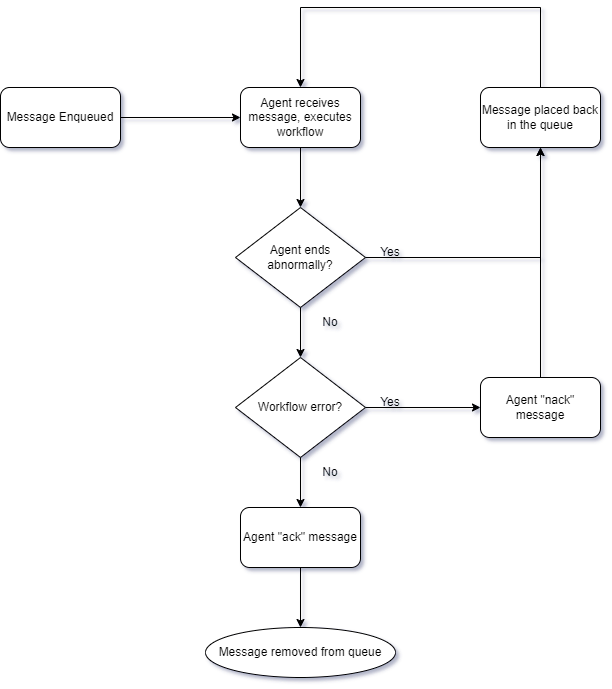
\includegraphics[width=\textwidth]{graphics/cxoneflow-diagrams-Recovery Algorithm.png}
    \caption{Workflow Recovery Algorithm}
    \label{fig:recovery-flowchart}
\end{figure}



\section{Scan Monitoring}

A scan in CheckmarxOne can be performed using one or more different scan engines.
A scan that has been completed will generally decide the next step in the workflow.
Keep in mind that a "completed" scan may mean the scan ended with any of the
following outcomes:

\begin{itemize}
    \item Scans for all requested engines completed successfully, each having zero
    or more results.
    \item The scan may have failed with no engines ever having started a scan.
    \item The scan may have partially failed where one or more engines successfully
    completed a scan and one or more engines had a scan failure.
    \item The scan may have been cancelled before any engine produced results.
    \item The scan may have been cancelled after one or more engines produced
    results but before all the engines were able to produce results.
\end{itemize}

When the scan is completed (which doesn't imply that it was successful), a message
is enqueued that starts the next step in the workflow.  
Figure \ref{fig:polling-flowchart} shows the scan polling algorithm that is followed
to determine when to enqueue a message that starts the next step in the workflow.

\begin{figure}[ht]
    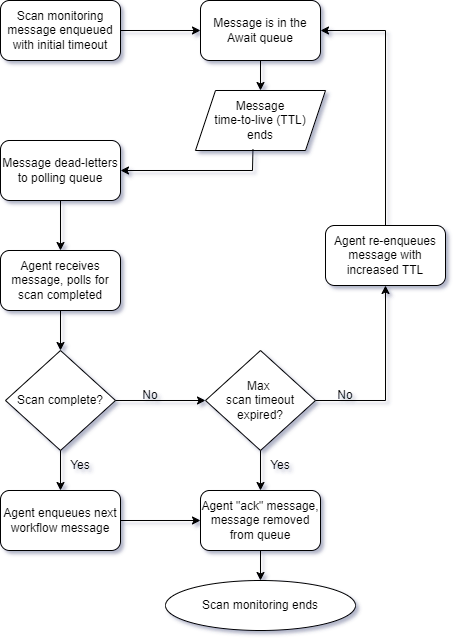
\includegraphics[width=\textwidth, scale=.75]{graphics/cxoneflow-diagrams-Polling Algorithm.png}
    \caption{Scan Polling Algorithm}
    \label{fig:polling-flowchart}
\end{figure}

\section{Annotation Workflow}\label{sec:annotation-workflow}

The annotation workflow is intended to perform any type of operations that
would inform a user of the following scan dispositions:

\begin{itemize}
    \item Started
    \item Cancelled
    \item Failed
\end{itemize}

\noindent\\The messaging workflow is currently very simple and follows the algorithm
shown in Figure \ref{fig:recovery-flowchart}.

\section{Pull Request Feedback Workflow}\label{sec:pull-request-workflow}

The pull request feedback workflow is invoked when a scan completes with the
following conditions:

\begin{itemize}
    \item A scan is fully completed on all requested scan engines.
    \item A scan is in the \texttt{Partial} result state with no
    engines currently running a scan.
\end{itemize}

The feedback workflow messaging follows the algorithm shown in
Figure \ref{fig:recovery-flowchart}.  The feedback that is emitted
for pull-request feedback is a summary of components found in the
\href{https://docs.checkmarx.com/en/34965-182434-checkmarx-one-reporting.html}{Improved Scan Report}
as generated by the
\href{https://checkmarx.stoplight.io/docs/checkmarx-one-api-reference-guide/branches/main/7bf86350cfe72-create-a-report}{"create a report"}
CheckmarxOne API.  Some results can be excluded via configuration,
as described in Section \ref{sec:exclusions-element}.  If the results of a particular
engine are not included in the Improved Scan Report, they are not available for
publication in the feedback comment.

\subsection{Pull Request Comment Contents}

Each source control system will impose a maximum size for content written in
a pull request comment.  Since scans can produce an unpredictable number of
results for each engine scanned, it is possible that a full itemized
summary of results in a pull request comment will exceed the maximum comment
size.  \cxoneflow will write the full itemized summary of results if the
content size is less than the maximum comment content size.  In the event that
the maximum comment content size would be exceeded, a simple count of
vulnerabilities by severity and engine is written as the comment content.


\subsubsection{Header}

An example header of the pull-request comment is shown in Figure
\ref{fig:pr-header-section}.  It contains a link to the scan
and an indicator of the scan status of the selected engines.  An indicator
of a red "X" next to an engine indicates the scan status of anything other
than successful completion of the scan running on that engine.

\begin{figure}[ht]
    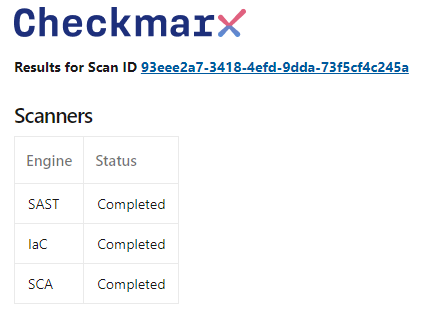
\includegraphics[width=\textwidth]{graphics/pr-header.png}
    \caption{Pull-Request Comment Header}
    \label{fig:pr-header-section}
\end{figure}

\subsubsection{Summary of Vulnerabilities}

An example summary of vulnerability counts by severity and engine 
is shown in Figure \ref{fig:pr-summary}.  The calculated counts will not
include vulnerabilities marked as "Not Exploitable".  Severities that
are configured for exclusions, as documented in Section
\ref{sec:exclusions-element}, are not included in the table.  When no 
vulnerabilities of a given severity with a status other than 
"Not Exploitable" are found, the count is indicated by "N/R" (none reported).


The counts for SCA scans only reflect the reported vulnerabilities in the
Risks tab of the SCA results viewer.  The count will differ from the summary
of SCA results shown when selecting a scan in Scan History; the scan
history view shows a combined count of all categories of SCA results.

\begin{figure}[ht]
    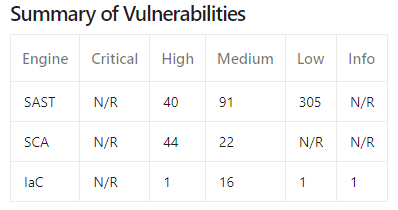
\includegraphics[width=\textwidth]{graphics/pr-summary.png}
    \caption{Pull-Request Summary Count by Severity and Engine}
    \label{fig:pr-summary}
\end{figure}


\subsubsection{SAST Results}

An example of the SAST result summary written to the pull-request comment
is shown in Figure
\ref{fig:pr-sast-section}.  The name of the issue is a link to a detailed
explanation of the vulnerability that includes remediation advice.  A
link to the line of the source code leads to the source file located in the
repository.  The Checkmarx Insight link opens the triage view for the vulnerable
data flow.

\begin{figure}[ht]
    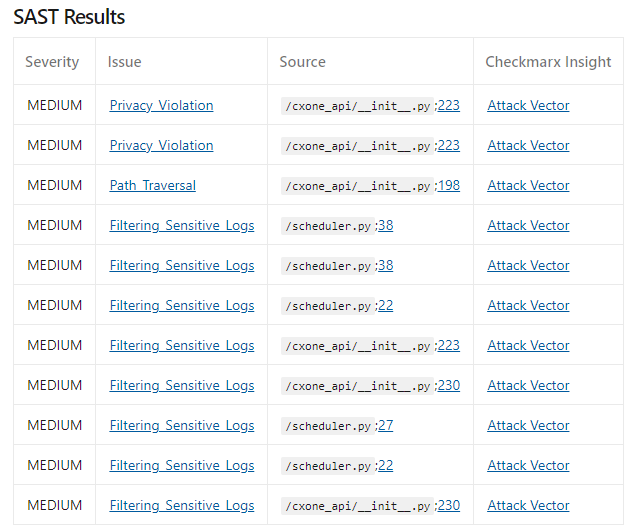
\includegraphics[width=\textwidth]{graphics/pr-sast.png}
    \caption{Pull-Request Comment SAST Results}
    \label{fig:pr-sast-section}
\end{figure}

\subsubsection{SCA Results}

An example of the SCA result summary written to the pull-request comment
is shown in Figure
\ref{fig:pr-sca-section}.  The Checkmarx Insight link opens the triage view 
for the vulnerable package. 

\begin{figure}[ht]
    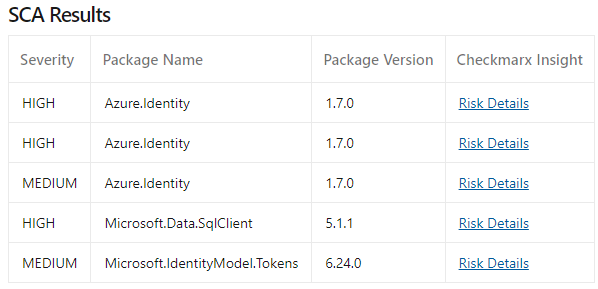
\includegraphics[width=\textwidth]{graphics/pr-sca.png}
    \caption{Pull-Request Comment SCA Results}
    \label{fig:pr-sca-section}
\end{figure}

\subsubsection{IAC Results}

An example of the IAC result summary written to the pull-request comment
is shown in Figure
\ref{fig:pr-iac-section}. A
link to the line of the source code leads to the source file located in the
repository.  The Checkmarx Insight link opens the triage view for the vulnerable
configuration.

\begin{figure}[ht]
    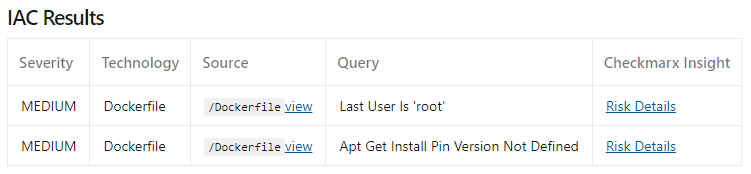
\includegraphics[width=\textwidth]{graphics/pr-iac.png}
    \caption{Pull-Request Comment IaC Results}
    \label{fig:pr-iac-section}
\end{figure}

\subsubsection{Resolved Issues}

An example of the Resolved Issues summary written to the pull-request comment
is shown in Figure
\ref{fig:pr-resolved-section}. This section appears only if a scan results in
some of the issues are found to have been resolved by a new scan.
The Checkmarx Insight link opens the triage view for the vulnerable
data flow.

\begin{figure}[ht]
    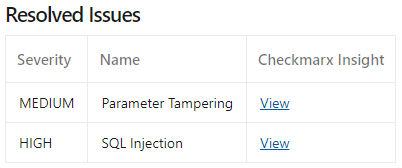
\includegraphics[width=\textwidth]{graphics/pr-resolved.png}
    \caption{Pull-Request Comment Resolved Section}
    \label{fig:pr-resolved-section}
\end{figure}

